%\documentclass[a4paper]{article}
%\usepackage{beamerarticle}

\documentclass[ignorenonframetext]{beamer}
\usepackage{beamerthemesplit}
\usepackage{amssymb}

\usepackage{../fhnw-beamer}

%\mode<article>{\usepackage{fullpage}}
%\mode<presentation>{\usetheme{Berlin}}

\date{\today}
\author{rolf.schmutz@fhnw.ch}
\institute{FHNW}
\title{Netzwerke und Kommunikation\\B-LS-MI 004\\Homework: Network Address Translation\\NAT}


\begin{document} % ===============================================================

\section{B-LS-MI 004: NAT}



\begin{frame}
\titlepage
\end{frame}




\begin{frame}
\frametitle{Ziele}
\begin{itemize}
	\item Sie kennen die Verwendung der RFC1918 {\em private addresses} und die dazu n\"otigen Vorkehrungen
	  \item $\ldots$die Adressbereiche
	  \item die n\"otige Statustabelle
	  \item die ``Vorschriften'' zur Verwendung
	  \item die Einsatzm\"oglichkeiten
\end{itemize}
\end{frame}




\begin{frame}
\frametitle{IPv4 Adressenknappheit}
\begin{center}
	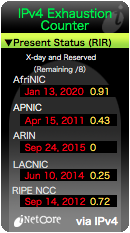
\includegraphics[height=5cm]{ipv4-exhaustion-counter}\\
\end{center}
\myurl{http://inetcore.com/project/ipv4ec/en-us/index.html}

$\rightarrow$ IPv4-Adressen sind eine sehr knappe Resource
\end{frame}



\begin{frame}
\frametitle{IPv4 Adressenknappheit Problem}
\begin{itemize}
	\item{Grosse Adressbl\"ocke werden intern\footnote{d.h. werden im Internet nicht ``geroutet'' und sind somit nicht eigentlich Bestandteil des Internets $\rightarrow$ Verschwendet\\z.B. die Schweizerische Post: 138.191/16=intern, Apple Inc 17/8 meist intern verwendet} verwendet}
	\item{Traditionell reservierte Bl\"ocke\footnote{z.B. 127/8, 0/8, etc}}
\end{itemize}
$\rightarrow$ eigentlich noch viele Adressen ``frei'' aber nicht zur \"offentliche Nutzung 
\\
\vspace{1cm}
Update/2020:

Die Situation mit den ``grossen privaten'' Adressbl\"ocken hat sich entspannt/verlagert:
\begin{itemize}
  \item grosse Netzwerke wurden freigegeben (1/8, 8/8, 9/8, 3/8, 5/8, etc)
  \item $\ldots$und wurden gleich wieder von grossen Akteuren\footnote{z.B. Cloud-Infrastruktur-Betreiber, die Verwendung ist aber \"ahnlich wie bei Internet-Service-Provider} ``geschluckt''
\end{itemize}
\end{frame}




\begin{frame}
\frametitle{IPv4 Adressenknappheit L\"osung\footnote{sort of$\ldots$}: {\em private networks}}
\begin{itemize}
	\item{Reine Client-Computer\footnote{Arbeitsstationen zum surfen, mailen, etc} m\"ussen {\em aus} dem Internet nicht sichtbar sein\footnote{Bzw. der Verbindungsaufbau geht immer {\em von} diesen Computer aus}}\\$\rightarrow$ diese Adressen m\"ussen nicht eindeutig sein
	\item{Um trotzdem das korrekte Routing im Internet sicherzustellen {\em m\"ussen} solche Adressen sp\"atestens beim Verbindungsrouter ins Internet in eine {\em \"offentliche}{}\footnote{{\em public}} IP-Adresse umgewandelt werden}
	\item{das private Netzwerk wird gegen\"uber dem Internet hinter einer\footnote{oder mehrere$\ldots$} {\em \"offentlichen} Adresse ``verborgen''}
\end{itemize}
$\rightarrow$ drei Netzwerke sind in RFC1918\footnote{\myurl{http://www.rfc-editor.org/rfc/pdfrfc/rfc1918.txt.pdf}} zur {\em internen} Verwendung freigegeben:
\begin{center}
\begin{tabular}{|c|}
\hline
192.168.0.0/16 \\
172.16.0.0/12 \\
10.0.0.0/8 \\
\hline
\end{tabular}
\end{center}
\end{frame}




\begin{frame}
\frametitle{NAT: ``Vorschriften''}
\begin{itemize}
	\item die drei RFC1918-Bereiche 10/8, 172.16/12 und 192.168/16 d\"urfen uneingeschr\"ankt in einem privaten/lokalen Netzwerk-Verbund benutzt werden
	\item es darf nie eine solche Adresse ``ins Internet'' gelangen -- d.h. in den 
	\"offentlichen Teil des Internets\footnote{source: Antwort/R\"uckweg w\"urde nicht funktionieren, destination: kann nicht in Routing-Tables im Internet gefunden werden (per Definition)}
\end{itemize}
\end{frame}



\begin{frame}
\frametitle{NAT: Spielarten}
\begin{itemize}
	\item{``Masquerading'': n:1 dynamisches NAT\footnote{also PAT, port-address-translation}, one-way. Das, was Sie zuhause benutzen}
	\item{static n:n oder n:m NAT: feste Zuordnung\footnote{$\ldots$dies spart nat\"urlich keine public-IPs} von {\em private} zu {\em public} Adressen}
	\item{dynamic n:m NAT\footnote{das ist in der FHNW f\"ur Clients so eingerichtet}: ein (gr\"osserer) {\em private} Bereich wird auf einen (kleineren) {\em public} Bereich ``gemappt''}
	\item{PAT\footnote{$\ldots$ja, da herrscht ein wenig Begriffsverwirrung. Viele Hersteller von SOHO-Router (Zyxel, Netgear, etc) benutzen diese Terminologie}, port-address-translation: wie {\em masquerading} aber mit spezifischen Umleitungen von {\em eingehenden} Verbindungen auf spezielle Ports zu festen {\em private} Adressen\footnote{z.B. um zuhause auf einem PC mit {\em private} Adresse einen Webserver zu betreiben}}
\end{itemize}
\end{frame}




\begin{frame}
\frametitle{NAT: Problemstellung}
\begin{itemize}
	\item{Ausgehende {\em private} IP-Adressen m\"ussen auf {\em public} umgeschrieben werden}
	\item{bei eingehenden Paketen muss die Zieladresse\footnote{das ist die im ersten Schritt eingesetzte {\em public} Adresse} vor der Weiterleitung in das interne Netz wieder in die entsprechende {\em private} Adresse umgeschrieben werden}\\
	$\rightarrow$ d.h. wir brauchen eine Statustabelle
	\item{Eintr\"age in der Statustabelle m\"ussen {\em eindeutig} aus den eingehenden Paketen identifiziert werden k\"onnen}\\
	$\rightarrow$ dazu wird meistens ein 5 Tuple:\\
	{\small \{protocol, local-translated-ip, local-translated-port, remote-ip, remote-port\}}\\
	verwendet
	\item{Statuseintr\"age werden bei TCP nach Verbindungsabbau, bei UDP nach einer konfigurierbaren Zeitspanne gel\"oscht}
	\item{eingehende Pakete ohne passenden Eintrag in der Statustabelle werden verworfen}
\end{itemize}
\end{frame}



\begin{frame}
\frametitle{IPv4 NAT -- {\em Masquerading}}
\vspace{1cm}
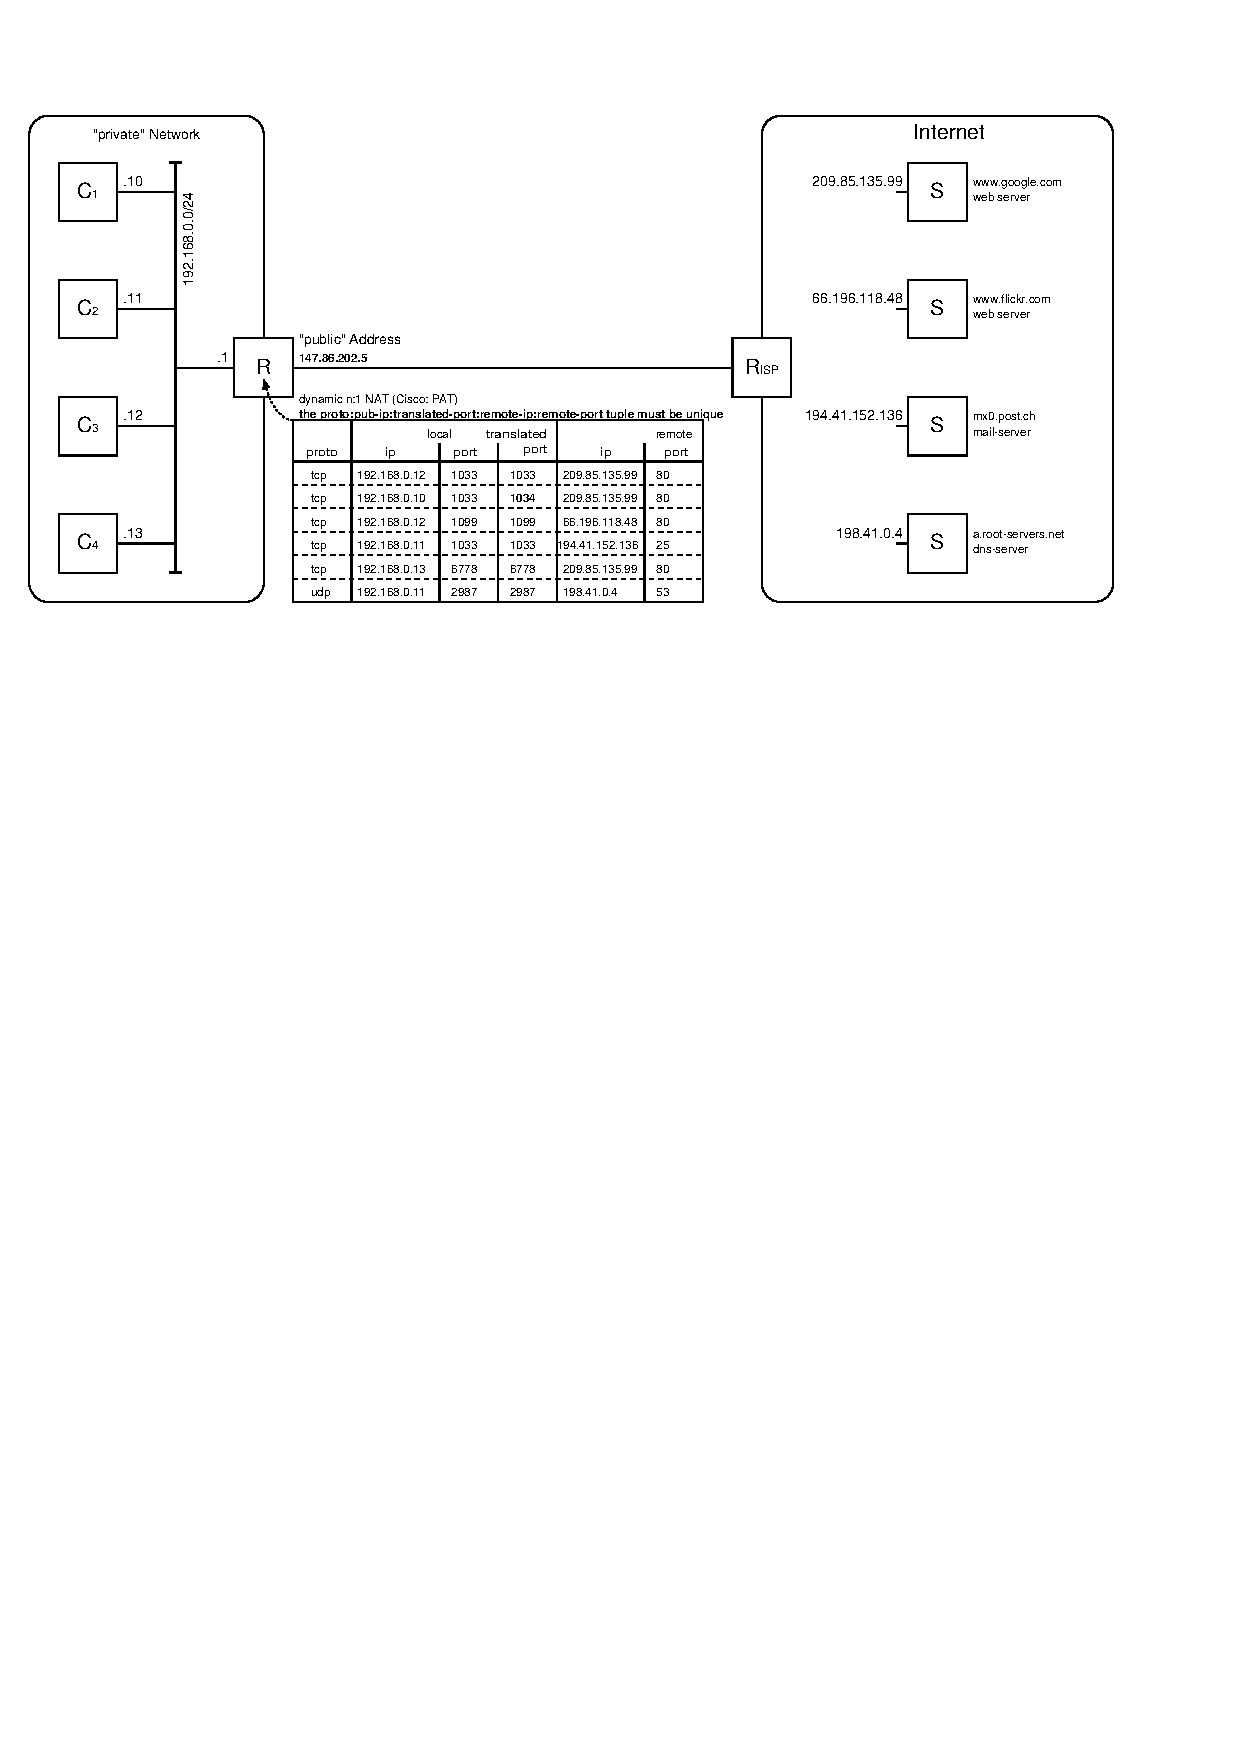
\includegraphics[height=18cm]{private-network}
\end{frame}



\begin{frame}
\frametitle{IPv4 NAT -- {\em Masquerading}}
\begin{itemize}

  \item man beachte den m\"oglichen Konflikt und die L\"osung durch Ersetzen des Source-Ports f\"ur den \"offentlichen Teil (Zeile 2)

  \item eine solche Statustabelle dient auch als {\em einfache} ``Firewall'':

  \begin{itemize}
     \item es werden nur Pakete entgegengenommen, die in der Tabelle einer Verbindung zugeordnet werden k\"onnen
     \item die Eintr\"age in der Tabelle erfolgen nur bei ausgehenden Verbindungen
     \item d.h. keine ``unzuweisbaren''/unaufgeforderte Pakete k\"onnen in das private Netzwerk gelangen

   \end{itemize}

\end{itemize}
\end{frame}







\begin{frame}[fragile]
\frametitle{NAT: Beispiel GNU/Linux (edited)}
	\begin{tiny}
		\begin{verbatim}
root@zaphod:~# cat /proc/net/ip_conntrack
udp      17 136   src=188.40.65.199 dst=109.75.190.27 sport=123 dport=123
                  src=109.75.190.27 dst=188.40.65.199 sport=123 dport=123 [ASSURED]
tcp      6 431999 ESTABLISHED
                  src=77.56.89.75 dst=188.40.65.199 sport=1104 dport=22 
                  src=188.40.65.199 dst=77.56.89.75 sport=22 dport=1104 [ASSURED]
tcp      6 344782 ESTABLISHED
                  src=77.56.89.75 dst=188.40.65.199 sport=8994 dport=22 
                  src=188.40.65.199 dst=77.56.89.75 sport=22 dport=8994 [ASSURED]
udp      17 16    src=188.40.65.199 dst=213.165.64.1 sport=6449 dport=53
                  src=213.165.64.1 dst=188.40.65.199 sport=53 dport=6449
icmp     1 20     src=188.40.65.199 dst=207.46.19.190 type=8 code=0 id=32527 [UNREPLIED] 
                  src=207.46.19.190 dst=188.40.65.199 type=0 code=0 id=32527
tcp      6 431979 ESTABLISHED
                  src=212.60.51.243 dst=188.40.65.199 sport=54054 dport=80 
                  src=188.40.65.199 dst=212.60.51.243 sport=22 dport=54054 [ASSURED]
tcp      6 261956 ESTABLISHED
                  src=77.56.89.75 dst=188.40.65.199 sport=7120 dport=22
                  src=188.40.65.199 dst=77.56.89.75 sport=22 dport=7120 [ASSURED]
udp      17 14    src=188.40.65.199 dst=62.219.186.11 sport=27015 dport=53 
                  src=62.219.186.11 dst=188.40.65.199 sport=53 dport=27015
tcp      6 13501 ESTABLISHED
                  src=77.56.89.75 dst=188.40.65.199 sport=40459 dport=22
                  src=188.40.65.199 dst=77.56.89.75 sport=22 dport=40459 [ASSURED]
udp      17 7     src=188.40.65.199 dst=188.40.65.199 sport=53745 dport=53 
                  src=188.40.65.199 dst=188.40.65.199 sport=53 dport=53745
tcp      6 8 TIME_WAIT
                  src=41.117.24.238 dst=188.40.65.199 sport=63745 dport=25 
                  src=188.40.65.199 dst=41.117.24.238 sport=25 dport=63745 [ASSURED]
tcp      6 425142 ESTABLISHED
                  src=71.103.253.162 dst=188.40.65.199 sport=4017 dport=25 [UNREPLIED]                   
                  src=188.40.65.199 dst=71.103.253.162 sport=25 dport=4017
		\end{verbatim}
	\end{tiny}
\end{frame}




\begin{frame}
\frametitle{NAT: neue Probleme$\ldots$}
\begin{itemize}
	\item{Protokolle, die IP-Adressinformationen als {\em payload}{}\footnote{in den Nutzdaten} transportieren m\"ussen speziell behandelt werden}\\
	$\rightarrow$ d.h. zus\"atzlich zu den Adressen im IP-Header m\"ussen auch die Adressen {\em im} Paket umgeschrieben werden\\
	Beispiele: FTP, SIP\footnote{Session-Initiation-Protocol, IP-Telefonie}
	\item{manche Protokolle haben keine Portnummern, die umgeschrieben oder in der Statustabelle eingetragen werden k\"onnen: ICMP}\\
	$\rightarrow$ durch die Paarung \texttt{protocol=ICMP} im Tuple wird meistens trotzdem eine eindeutige Zuweisung erreicht
\end{itemize}
\end{frame}


%\begin{frame}
%\frametitle{NAT: Network Address Translation}
%\end{frame}




\begin{frame}
\frametitle{References}
\begin{itemize}
	\item{NAT: \myurl{http://en.wikipedia.org/wiki/Network_address_translation}}
	\item{private address space \myurl{http://www.rfc-editor.org/rfc/pdfrfc/rfc1918.txt.pdf}}
\end{itemize}
\end{frame}





\end{document}